We begin with Navier-Stokes for an incompressible fluid:
\begin{equation} \label{eq:NS}
  \frac{\partial u_i}{\partial t} + u_k \frac{\partial u_i}{\partial x_k} = -\frac{\partial P}{\partial x_i} + \nu \frac{\partial^2 u_i}{\partial x_k \partial x_k}
\end{equation}
then, as the velocity gradient tensor is defined as $A_{ij} = \frac{\partial u_i}{\partial x_j}$, we apply spatial derivatives, and use the definition of material derivative ($\frac{dA_{ij}}{dt} = \frac{\partial A_{ij}}{\partial t} + u_k\frac{\partial A_{ij}}{\partial x_k}$) to get:
\begin{equation}
  \frac{dA_{ij}}{dt} = \frac{\partial A_{ij}}{\partial t} + u_k \frac{\partial A_{ij}}{\partial x_k} = - A_{ik}A_{kj} - \frac{\partial^2 P}{\partial x_i \partial x_j} + \nu \frac{\partial^2 A_{ij}}{\partial x_k \partial x_k}
\end{equation}
Additionally, from incompressibility, we have
\begin{equation}
  \frac{\partial^2 P}{\partial x_k \partial x_k} = - A_{ij}A_{ji}
\end{equation}
This allows us to define the nonlocal deviatoric part of the pressure hessian
\begin{equation}
  H_{ij} = - \left( \frac{\partial^2 P}{\partial x_i \partial x_j} - \frac{1}{3}\frac{\partial P}{\partial x_k \partial x_k}\delta_{ij}  \right)
\end{equation}

We can write the formal (nonlocal) solution for the deviatoric pressure hessian as\cite{ohkitani1995}

\begin{equation}
  H_{ij}(\textbf{x}) = \iiint \frac{\delta_{ij} - \hat{r_i}\hat{r_j}}{2\pi r^3}Q(\textbf{x} + \textbf{r})d\textbf{r}
\end{equation}

Following Lawson \& Dawson\cite{lawson2015}, an expansion of the integral is proposed, first as a Taylor series expansion in $Q(x+r)$
\begin{equation}
  \hat{H} = \sum_{m,n = 0}^\infty \alpha_{mn}S^mW^n
\end{equation}
where
\begin{equation}
  S = \frac{1}{2}(A + A^T) \qquad W = \frac{1}{2}(A - A^T)
\end{equation}

Finally we can reduce from an infinite sum using Cayley-Hamilton, and expand via the tensor basis\cite{zheng1993}
\begin{equation}
  \hat{H} = \sum_{n=1}^{10} g^{(n)}(\lambda_1, \dots, \lambda_5)T^{(n)}
\end{equation}
with $g^{(n)}$ scalar functions of the invariants
\begin{small}
  \begin{equation*}
    \lambda_1 = \tr(S^2) \quad \lambda_2 = \tr(W^2) \quad \lambda_3 = \tr(S^3) \quad \lambda_4 = \tr(W^2S) \quad \lambda_5 = \tr(W^2S^2)
  \end{equation*}
\end{small}
and the tensor basis given by:
\begin{small}
  \begin{align*}
    &T^{(1)} = S &T^{(2)} &= SW-WS\\
    &T^{(3)} = S^2 - \frac{1}{3}I \cdot \tr(S^2) &T^{(4)} &= W^2 - \frac{1}{3}I \cdot \tr(W^2)\\
    &T^{(5)} = WS^2 - S^2W &T^{(6)} &= W^2S + SW^2 - \frac{2}{3}I \cdot \tr(SW^2)\\
    &T^{(7)} = WSW^2-W^2SW &T^{(8)} &= SWS^2 - S^2WS\\
    &T^{(9)} = W^2S^2 + S^2W^2 - \frac{2}{3}I \cdot \tr(S^2W^2) &T^{(10)} &= WS^2W^2 - W^2S^2W
  \end{align*}
\end{small}
We use the natural timescale $\tau = \langle \norm{S^2}_2 \rangle^{-1}$ to normalize our VGT, and thus all of the $\lambda_i, T^{(j)}$.
This formulation reduces the challenge to finding the functions of known scalars, i.e., learning the $g^{(n)}$'s.

\begin{equation}
  \hat{H} = \sum_{i=1}^{10} g_{\theta}^{(i)}(\lambda_1, \dots, \lambda_5)\cdot \hat{T}^{(i)}(\hat{A})
\end{equation}

\begin{small}
  \begin{equation*}
    \lambda_1 = \tr(\hat{S}^2) \quad \lambda_2 = \tr(\hat{W}^2) \quad \lambda_3 = \tr(\hat{S}^3) \quad \lambda_4 = \tr(\hat{W}^2\hat{S}) \quad \lambda_5 = \tr(\hat{W}^2\hat{S}^2)
  \end{equation*}
\end{small}
\begin{figure}
  \centering
  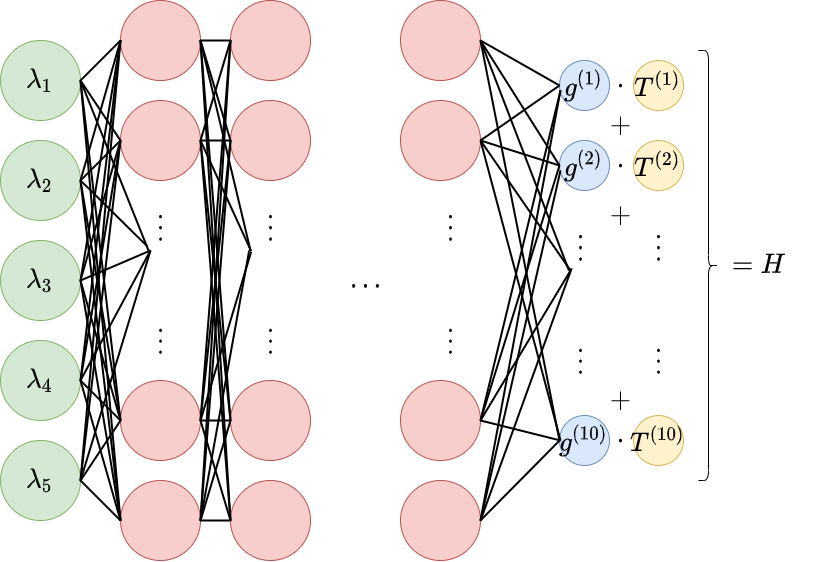
\includegraphics[width=0.5\textwidth]{./tbnn.png}
  \caption{Structure of TBNN}
  \label{fig:tbnn}
\end{figure}

\begin{equation}
  L(\theta) = \frac{1}{N}\sum^N\norm{\hat{H}_{\text{truth}} - \sum_{i=1}^{10}g_\theta^{(i)}(\lambda_1, \dots, \lambda_5)T^{(i)}}_2^2
\end{equation}


